%
% Uvod
%

\chapter{Úvod}

Každý linuxový server alebo osobný počítač môže slúžiť na niečo iné. Preto je
veľmi náročné vytvoriť linuxovú distribúciu, ktorá by pokrývala požiadavky
každého a~bola optimalizovaná pre všetky operácie. Preto je potrebné systém
nastaviť tak, aby presne vyhovoval naším potrebám a~získali sme maximálny výkon
pre naše potreby. Kedže sa jedná a~množstvo druhov nastavení, vznikol balíček
\emph{tuned}\cite{tunedHomepage}, ktorý ich zahrňuje.

Cieľom tejto práce je priblížiť \emph{tuned}, zhrnúť jeho hlavné funkcie,
popísať profily a~na záver implementovať sadu testov pre I/O operácie nad
najpoužívanejšími súborovými systémami a~diskovými zariadeniami. Na záver budú
testy spustené a~výsledky vyhodnotené.

%
% Popis komponenty
%

\chapter{Popis komponenty tuned}

Balíček \emph{tuned} je primárne napísaný pre linuxovú distribúciu
Fedora\cite{fedoraHomepage} a~Red Hat Enterprise Linux. Démon \emph{tuned} neustále
beží, skenuje systém a~upravuje nastavenia podľa potreby. Napríklad najväčšia
záťaž na disk je pri štarte systému alebo pri ukladaní dát na disk (napríklad
filmov). Inak je disk skoro nečinný. \emph{tuned} dokáže optimalizovať zápis práve v
tej dobe, keď je to potreba. Rovnako je to aj pri sieťových operáciach.

Niektoré profily zamedzujú aj prepínaniu Cx stavov \footnote{Cx sú stavy, v
ktorých sa môže vyskytovať procesor, typicky firmy Intel. Tieto stavy sa volajú
Spiacie stavy (ang. Sleep states) \cite{sleepStates}. Spiace stavy procesoru
slúžia na šetrenie energie.}.

Súčasťou \emph{tuned} je aj program \emph{tuned-adm}, ktorý nám dovoľuje
prepínať medzi profilmi. Každý z~profilov slúži na iné zameranie a~napriamo
podľa toho upravuje systém, čím dosahujeme ešte lepšie výsledky.

%
% Historia tuned
%

\section{História \emph{tuned}}
\label{sec:historiaTuned}

Komponenta \emph{tuned} je vyvýjaná od roku 2008. Prvými autormi boli
\emph{Philip Knirsh} a~\emph{Thomas WoVerner}. Dnes sú najväčšími
prispievatelia \emph{Ján Včelák}, \emph{Jaroslav Škarvada} a~\emph{Ján Kaluža}.
Dnes je \emph{tuned} vo verzii \emph{2}. Medzi verziou \emph{1} a~\emph{2} je
veľký rozdiel, pretože bol celý kód od základov prepísaný. Jedna z~najväčších
zmien je v~používaní \emph{D-BUS} \footnote{Systém pre jednoduché zasielanie
správ a~komunikáciu medzi aplikáciami}. Ďalšia zmena je v~profiloch. Niektoré
profily boli zmenené alebo odobraté. Pre zachovanie spätnej kompatibility
vznikol preto balík \emph{tuned-profiles-compat}, ktorý obsahuje všetky profily
z verzie \emph{tuned 1}.

%
% Profily tuned
%

\section{Profily}

Profily su hlavne zamerané na CPU, disky, sieť a~FSB \footnote{Front-Side Bus -
datová zbernica, ktorá zaisťuje komunikáciu medzi CPU a~hardvérom. Využíva sa v
procesoroch \emph{Intel}}. Samotný balíček obsahuje niekoľko predvolených
profilov a~ako základný profil je po spustení \emph{tuned} profil \emph{balanced}.

Profily si môžeme aj samy vytvárať. Ak si nie sme istý, čo je potrebné upraviť,
môžeme využiť odporúčania z~programu \emph{powertop}\cite{powertopHomepage}~a
za pomoci skriptu \emph{powertop2tuned} si nechať profil vytvoriť automaticky
na základe výstupu z~\emph{powertop}. Bližšiemu popisu profilov sa venuje
sekcia \ref{sec:prehladProfilov}. 


%
% Prehlad profilov
%

\subsection{Prehľad profilov}
\label{sec:prehladProfilov}

Profily \emph{tuned} sa nachádzajú v~adresári \emph{/usr/lib/tuned}. V~tomto
adresári sa taktiež nachádza súbor s~funkciami, ktoré tieto profily využívajú.
Práve tieto súbory sú najviac vyvýjané a~menené.

Prehľad profilov zo základného balíčka \emph{tuned}. Zoznam je platný pre
verziu \texttt{tuned-2.2.2-1} na \emph{Fedora 18}:

\begin{itemize}
    \item \textbf{balanced} -- predvolený profil pre väčšinu systémov s~výnimkou virtuálnych
    \item \textbf{latency-performance} -- znižuje latenciu systému
    \item \textbf{powersave} -- na zníženie odberu energie
    \item \textbf{throughput-performance} -- vylepšuje celkovú priepustnosť systému 
    \item \textbf{virtual-guest} -- predvolený profil pre virtuálne systémy
    \item \textbf{virtual-host} -- vhodný pre systémy, na ktorých sa prevádzkujú virtuálne systémy
\end{itemize}

Balíček \emph{tuned-profiles-compat} rozširuje zoznam o~tieto ďalšie profily:

\begin{itemize}
    \item \textbf{default}
    \item \textbf{desktop-powersave}
    \item \textbf{enterprise-storage}
    \item \textbf{laptop-ac-powersave}
    \item \textbf{laptop-battery-powersave}
    \item \textbf{server-powersave}
    \item \textbf{spindown-disk}
\end{itemize}

Medzi najčastejšie operácie profilov patrí menenie governoru\footnote{Rýchlosť
procesora je možné meniť a~tým šetriť energiu v čase, keď ho naplno
nevyužívame. Túto rýchlosť ovplyvňujú rôzne druhy plánovačov.} procesoru medzi
\texttt{ondemand}|\footnote{Nastavuje rýchlosť procesora podľa využitia.}
a~\texttt{performance}\footnote{Nastaví rýchlosť procesora na najvyššiu hodnotu
bez ohľadu na využitie.}. Viac o~tejto vlastnosti je možné dočítať sa na wiki
stránkach Arch Linuxu\cite{arch:governor}.

Ďalej je to nastavovanie plánovačov diskov. Toto nastavenie sa mení v~súbore
\texttt{/sys\-/block\-/<dev>\-/queue\-/scheduler}. Niektoré profily ho prepínajú z
predvoleného plánovača na \emph{deadline}\footnote{Tento plánovač sa používa
pre zníženie latencie. Obsahuje dve fronty a~každá požiadavka má deadline}.
Viac o~plánovačoch diskov je možné sa dočítať na stránkach dokumentácie
\emph{OpenSuse}\cite{suse:scheduler} alebo v článku \cite{book:scheduler}.

Niektoré profily taktiež vypínajú bpariéry\footnote{Vypnutím bariér hrozí
poškodenie dát pri odpojení napájania diskov, pokiaľ disk nemá záložnú
batériu.} pri pripojovaní diskov. 

%
% Emulacia diskovych zariadeni a sietovych sluzieb
%

\chapter{Emulácia diskových zariadení a sieťových služieb}

V tejto kapitole sa budem venovať emulácií diskových zariadení a sieťových
služieb v teoretickej rovine. Je potrebné si uvedomiť, že na to, aby bolo
testovanie na 100\,\% valídne nám emulácia nestačí a bolo by potrebné všetky
testovacie prostriedky mať k dispozícií, čo nie je možné.

Aj keby tomu tak bolo, nie je možné program dokonale otestovať, pretože
väčšinou existuje nekonečne veľa možností vstupu. V prípade testovania hardvéru
sa táto skutočnosť ešte násobi, kedže na neho môže vplývať ešte viac vplyvov
ako na softvér. Tejto myšlienke sa venuje aj \emph{Ron Patton} v Knihe
\emph{Software Testing} \cite{Software_testing_patton}, kde opisuje testovanie
obyčajnej kalkulačky.

\section{Sieťové služby}

Ak chceme testovať rôzne typy sietí, \emph{Linux} nám k tomu poskytuje sieťové
skripty, ktorými dokážeme vytvárať pomerne zložité návrhy sieti v rámci jedného
systému. Môžeme vytvárať mosty medzi zariadeniami, virtuálne podsiete a
podobne.

V prípade, že využijeme virtuálne systémy, sa dajú vytvoriť aj pokročilejšie
situácie a pri testovaní môžeme využívať služby na rôznych strojoch. Na webový,
emailový a DNS server môžeme použiť oddelené systémy a testovať ich navzájom.

Existuje množstvo hardvérových riešení pre emuláciu sietí. Tieto zariadenia ale
nie sú relevantné pre komponentu \emph{tuned}, pretože vyžaduje operačný systém
\emph{Fedora} alebo jemu podobné. Pri týchto riešeniach sa jedná ale väčšinou o
rôzne vstavané systémy.

Testovanie sietí je veľmi obsiahla téma a nie je zameraním tejto bakalárskej
práce.

%
% Diskove zariadenia
%

\section{Diskové zariadenia}

K emulácii diskových zariadení sa dá pristupovať dvoma spôsobmi. 

\begin{enumerate}
    \item Bez využitia virtuálneho systému \label{item:without-virt-system}
    \item S využítím virtuálneho systému \label{item:with-virt-system}
\end{enumerate}

%
% Bez vyuzitia virtualneho systemu
%

\subsection{Bez využítia virtuálneho systému}

Ak nechceme využiť virtuálny systém, potrebujeme vytvoriť blokové zariadenie
diskou bez toho, aby sme v skutočnosti pripojili fyzický disk. K tomu slúži
napríklad balíček \texttt{scsi-target-utils}, ktorý obsahuje nástroj
\texttt{/usr/bin/tgtadm}.  Tento nástroj dokáže vytvoriť \emph{SCSI} cieľový
disk aj zo súbora. 

Ďalej budeme potrebovať spustiť službu \texttt{tgtd}, ktorá nám takto pridaný
disk sprístupní na sieť. Tento prístup sa používa vtedy, keď potrebujeme takýto
disk nazdielať cez sieť. Samozrejme, môžeme ho pripojiť aj s využítím
\emph{localhost} PC.

Keď máme takýto disk prichystaný, pripojíme ho za pomoci príkazu uvedenénho v
algoritme \ref{alg:iscsiadm-discovery}. Tento nástroj sa nachádza v balíčku
\texttt{iscsi-initiator-utils}.
\\
\begin{lstlisting}[caption=Vyhľadávanie diskov na sieti pomocou iscsiadm,label=alg:iscsiadm-discovery]
    /usr/sbin/iscsiadm -m discovery -t st -p 127.0.0.1
\end{lstlisting}

Pre korektnosť pripojenia je vhodné premazať všetky nepoužité mapy zariadení.
Na to nám poslúži nástroj \texttt{/sbin/multipath} z balíčka
\texttt{device-mapper-multipath}. Aby sme ho mohli využiť, je taktiež potrebné
zaviesť do jadra modul \texttt{dm-multipath}. Potom je vhodné reštartovať celú
službu \texttt{multipathd}. Celý postup je uvedený v algoritme
\ref{alg:multipathd}.
\\
\begin{lstlisting}[label=alg:multipathd,caption=Vyhľadanie zariadení pomocou multipathd]
    modprobe dm-multipath
    /sbin/multipath -F
    /etc/init.d/multipathd restart
    multipath -ll
\end{lstlisting}

Keď som testoval tento typ pripojenia diskov, narazil som na problém s
načasovaním. Je potrebné nechať medzi príkazmi krátke časové intervaly na to,
aby všetko prebehlo korektne. Ak sa tieto príkazy spustia za sebou, je vysoká
pravdepodbobnosť, že sa disky nenájdu a nepripoja.

%
% S vyuzitim virtualneho systemu
%

\subsection{S využítím virtuálneho systému}

S virtuálnym systémom sa situácia zjednodušuje. Virtualizácia je v dnešnej dobe
veľmi pokročilá. Ak sa rozhodneme používať \emph{libvirt} a \emph{qemu-kvm},
tak existuje viacero nástrojov, ktoré nám uľahčujú prácu s virtuálnymi
systémami.

Pre tých, ktorí majú radi klikacie nástroje, existuje skoro dokonalý
\emph{virt-manager}. Vytvoriť si v ňom virtuálny systém a podrobne si ho
nastaviť je otázka niekoľkých kliknutí. 

Automatické testy ale nemôžu používať klikacie GUI nástroje. Preto existuje
nástroj \texttt{/bin/virsh} z balíka \texttt{libvirt-client}, ktorý dokáže
zjednodušene pracovať s virtuálnymi systémami z príkazovej riadky.  

Nastavenia virtuálneho stroja cez \emph{libvirt} sa ukladajú ako
\emph{XML}\footnote{eXtensible Markup Languagei -- rozšíriteľný značkovací
jazyk} dokument. Tieto konfiguračné súbory sú uložené štandardne v zložke
\texttt{/etc/libvirt/qemu} a majú ľahko pochopiteľnú štruktúru.

Ak chceme pridať nový disk, tak do pridáme nového potomka k uzlu
\texttt{<devices>}, ktorý môže vyzerať napríklad ako v ukážke
\ref{alg:libvirt-xml-disk}.
\\
\renewcommand{\lstlistingname}{Ukážka}
\begin{lstlisting}[label=alg:libvirt-xml-disk,caption=Príklad diskového zariadenia pre libvirt]
<disk type='file' device='disk'>
    <driver name='qemu' type='raw'/>
    <source file='/home/user/Virtuals/F18.img'/>
    <target dev='sda' bus='sata'/>
    <address type='drive' controller='0' bus='0' target='0' unit='0'/>
</disk>
\end{lstlisting}
\renewcommand{\lstlistingname}{\listingAlgoritmus}

Niektoré typy zariadení je možné pripájať dokonca aj počas behu virtuálneho
systému. Na to sa používa príkaz uvedený v \ref{alg:virsh-attach-device}.
\\
\begin{lstlisting}[label=alg:virsh-attach-device,caption=Pripojenie zariadenia bez priamej úpravy XML súbora]
/bin/virsh attach-device <názov stroja> súbor.xml
\end{lstlisting}

Treba brať na vedomie ale to, že takto pridané zariadenie je pripojené len do
najbližsieho vypnutia stroja, pretože tento príkaz neovplyvňuje hlavný XML
súbor stroja.

%
% Testovanie diskovych zariadeni a sietovych sluzieb
%

\chapter{Testovanie diskových zariadení a sieťových služieb}

Či už zariadenia máme fyzicky pripojené alebo ich len simulujeme, nemalo by to
mať vplyv na spôsob ich testovania.

%
% Testy pre sietove sluzby
%

\section{Testy pre sieťové služby}

V prvom rade je potrebné si rozmyslieť, čo konkrétne chceme zo sieťových
služieb testovať a uvedomiť si, čo všetko má na testovanie vplyv a obsiahnuť
všetky možnosti je nad rámec bakalárskej a asi aj diplomovej práce.

Ako príklad môžeme uviesť jednoduchý test -- meranie rýchlosti LAN siete.
Najjednoduchšia varianta, čo by mohla niekoho napadnúť je, merať rýchlosť
sťahovania pripraveného súbora cez HTTP protokol. Na jednom uzly siete sa
vytvorí server a na druhom uzly začneme sťahovanie. Toto riešenie ale nie je
úplne presné, kedže samotný protokol má taktiež nejakú réžiu. Preto treba ísť
na čo najnižšiu vrstvu a ideálne si spraviť vlastný merací nástroj, ktorý bude
pracovať priamo s packetmi. Na meranie ale má vplyv každé zariadenie, ktoré je
v ceste od jedného bodu k druhému.

%
% iperf
%

Na meranie výkonnosti siete existuje napríklad nástroj
\emph{iperf}\footnote{Domovská stránka -- http://iperf.sourceforge.net}
vyvýjaný \emph{NLANR/DAST}, ktorý dokáže merať priepustnosť siete, stratu
paketov a iné.  Projekt NLANR bohužial skončil pred pár rokmi a preto je
projekt neaktívny.  Posledná zmena na ňom bola v roku 2011.

\emph{Iperf} je potrebné spustiť na jednom systéme ako server a na druhom ako
klient. Príklad najjednoduchšieho použitia je v ukážke \ref{alg:iperf-usage}.
\\
\renewcommand{\lstlistingname}{Ukážka}
\begin{lstlisting}[label=alg:iperf-usage,caption=Príklad použitia iperf]
/bin/iperf -s # Spustenie ako server
/bin/iperf -c <host> # Spustenie ako klient, kde <host> je IP adresa servera
\end{lstlisting}
\renewcommand{\lstlistingname}{\listingAlgoritmus}

Výsledok takéhoto jednoduchého príkladu môže vyzerať napríklad ako v ukážke
\ref{alg:iperf-results}. Ako je vidieť, server mal IP adresu
\texttt{192.168.0.103} a program nameral rýchlosť 168\,Mbits/sec.
\\
\renewcommand{\lstlistingname}{Ukážka}
\begin{lstlisting}[label=alg:iperf-results,caption=Výstup z programu iperf]
-------------------------------------
Client connecting to 192.168.0.103, TCP port 5001
TCP window size: 22.9 KByte (default)
-------------------------------------
[  3] local 192.168.0.120 port 60573 connected with 192.168.0.103 port 5001
[ ID] Interval       Transfer     Bandwidth
[  3]  0.0-10.0 sec   201 MBytes   168 Mbits/sec
\end{lstlisting}
\renewcommand{\lstlistingname}{\listingAlgoritmus}

%
% TTCP
%

Ďalší nástroj, ktorý je možné použiť je \emph{PCATTCP}\footnote{PCAUSA Test TCP
-- http://www.pcausa.com/Utilities/pcattcp.htm}. Tento program má podporu aj
pre \emph{IPv6} a je vyvýjaný pre Windows. Jeho unixová varianta sa volá
\emph{Unix Test TCP}. 

\section{Testy diskových zariadení}

Meranie rýchlosti zápisu alebo čítania disku nie je až tak problematické, ak si dáme pozor na to, či zápis prebehol v skutočnosti alebo ešte len čaká vo vyrovnávacej pamäti. Najjednoduchší spôsob merania zápisu môžeme previesť nástrojom \texttt{/bin/dd}. Príklad použitia a jeho výsledku je možné vidieť v ukážke \ref{alg:dd-usage}.
\\
\renewcommand{\lstlistingname}{Ukážka}
\begin{lstlisting}[label=alg:dd-usage,caption=Príklad použitia a výsledok nástroja dd]
$ /bin/dd if=/dev/zero of=file bs=1M count=300 conv=fdatasync
300+0 records in
300+0 records out
314572800 bytes (315 MB) copied, 2.96816 s, 106 MB/s
\end{lstlisting}
\renewcommand{\lstlistingname}{\listingAlgoritmus}

Voľba \texttt{conv=fdatasync} nám zabezpečuje to, že \emph{dd} po zápise vyžiada synchronizáciu systému a tým sú dáta v skutočnosit naozaj zapísané na disk.

%
% Plan testovania
%

\chapter{Plán testovania pre Fedora Linux}

%\section{Test Plan Identifier}
%\section{References}

%\section{Introduction}
\section{Úvod}

Na testovanie tuned využijeme pomocnú knižnicu \emph{beakerlib}
\cite{beakerlibHomepage} pre jednoduchšie písanie testov a~prehľadnejšiu
interpretáciu dosiahnutých výsledkov. Cieľom testovania je zistiť, nakoľko
\emph{tuned} ovplyvňuje rýchlosť diskových operácií.

%\section{Test Items}
\section{Testovacie položky}

Napísané testy budú overovať správnu funkcionalitu \emph{tuned} démona a~taktiež
profilov v~zameraní na diskové operácie. Všetky testy budú
pripravené pre linuxovú distribúciu Fedora~18~\cite{fedoraHomepage}.

Overí sa rýchlosť zápisu na bežných aj RAID diskoch a~s~najpoužívanejšími
súborovými systémami uvedenými v~zozname nižsie.

\begin{itemize}
    \item ext2
    \item ext3
    \item ext4
    \item xfs
    \item jfs
    \item ReiserFS
    \item btrfs
\end{itemize}


%\section{Software Risk Issues}
\section{Softvérové riziká}
\label{sec:softverove-rizika}

V prípade zlyhania niektorých testov môže prísť k~poškodeniu už pripojených
diskov. Preto je vhodné spúšťat sadu testov na virtuálnom stroji. V~prípade
vydania novej verzie \emph{tuned} alebo inej použitej komponenty je tu riziko,
že testy nebudú stabilné a~môžu sa správať nepredvídateľne. V~tomto prípade ale
môžeme uvažovať o~nájdení chyby (dokonca regresie) v~\emph{tuned}.

%\section{Features to be Tested}
\section{Čo sa bude testovať}

Hostiteľský systém bude spúšťať predpripravené obrazy virtualizovaného systému
Fedora 18. K~virtualizovanému systému sa budú pripájať ďalšie disky. Tieto nové
disky budú formátované na najpoužívanejšie súborové systémy a~testované ich
rýchlosti pri rôznych profiloch \emph{tuned}.

Na testovacie účely použijeme najnovšiu verziu \emph{tuned} z~repozitára
\emph{Fedora 18}.

%\section{Features not to be Tested}
\section{Čo sa nebude testovať}

Pretože testy bežia na virtualizovanom hardvéri, výsledky môžu byť trocha
skreslené. Viac o~testovaní na virtualizovanom systéme v~kapitole
\ref{sec:virtual-machine}.

%\section{Approach}

%\section{Item Pass/Fail Criteria}
\section{Kritéria pre splnenie testov}

Počas testovania so zapnutým démonom \emph{tuned} by všetky I/O operácie diskov
mali byť rýchlejšie alebo aspoň tak rýchle ako s~vypnutým \emph{tuned}. Žiadna
operácia by nemala skončiť s~chybou a~disky by sa nemali poškodiť. Zápis so
zapnutým \emph{tuned} musí mať rovnaké výsledky ako s~vypnutým.

Výnimku tvoria len tie profily, ktoré nemajú za úlohu zvyšovať výkon. Medzi
tieto profily patrí napriklad \emph{powersave}, ktorý naopak môže diskové
operácie spomalovať.

%\section{Suspension Criteria and Resumption Requirements}
\section{Kritéria na prerušenie testovania}

Ak zlyhá operácia pripájania disku k~virtuálnemu stroju, ďalšie testovanie
stráca význam. Preto je potrebné počas testovanie kontrolovať, či táto kľúčová
operácia dopadla úspešne. Rovnaká situácia môže nastať, ak zlyhá nahratie
uloženého obrazu disku systému pred testovaním.

Prvý prípad (pripájanie obrazu disku) sa rieší opakovaním testu. Takto
dosiahneme vždy požadované výsledky, aj keď operácia zlyhá. Problém pripájania
diskov je bližšie popísaný v~sekcii \ref{sec:libvirt-problem}.

%\section{Test Deliverables}
\section{Čo obsahuje plán testovania a~jeho výsledky}

Celé testovania sa skladá z~niekoľkých súčastí:

\begin{itemize}
    \item Plán testovania.
    \item Zdrojové kódy jednotlivých testov.
    \item Knižnica na spracovanie výsledkov.
    \item Zoznam chýb, ktoré nastali.
    \item Vyhodnotenie výsledkov.
\end{itemize}

Výsledky testov majú podobu nameraných hodnôt v tabuľkách (generujú sa
automaticky) a písomného popisu týchto hodnôt.

%\section{Remaining Test Tasks}
%\section{Environmental Needs}
%\section{Staffing and Training Needs}
%\section{Responsibilities}
%\section{Schedule}
%\section{Planning Risks and Contingencies}
%\section{Approvals}
%\section{Glossary}

%
% Testovanie
%

\chapter{Príprava prostredia a implementácia testov}

\section{Nastavenia systému}

Pred testovaním je potrebné pripraviť si nainštalovaný systém \emph{Fedora 18}
ako obraz disku. Tento obraz sa bude spúšťať cez qemu-kvm. Disk, na ktorom sa
bude testovať rýchlosť zápisu a čítania by mal byť v~ideálnom prípade
nekešovaný.  Pred testovaním aj po testovaním je potrebné hostiteľský aj
virtualizovaný systém synchronizovať a~zmazať nakešované stránky (Algoritmus
\ref{alg:sync}).
\\
\begin{lstlisting}[caption=Synchronizácia systému,label=alg:sync]
    /bin/sync
    echo 3 > /proc/sys/vm/drop_caches
\end{lstlisting}

Každé miesto, kde je možnosť, že by systém si uchovával nejaké nakešované data,
ktoré by mohli ovplyvniť výsledky testovania je potrebné poznať (Obrázok
\ref{graf-cache}).

\begin{figure}[ht]
\begin{center}
  \makebox[\textwidth]{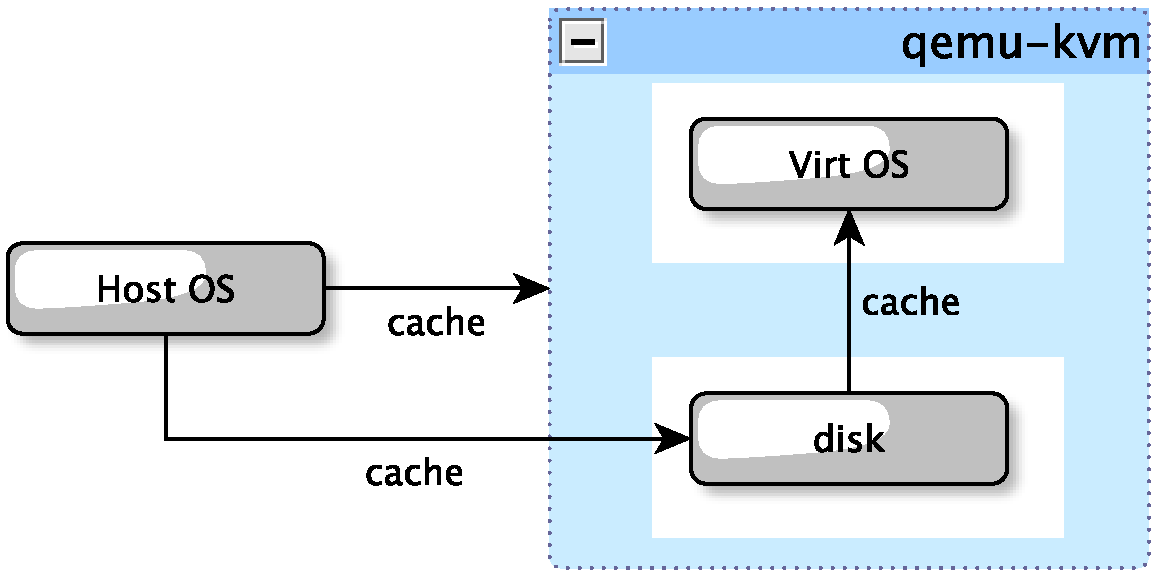
\includegraphics[width=\paperwidth/2]{data/cache.pdf}}
  \caption{Vyznačenie miest, kde môže nastať kešovanie}
  \label{graf-cache}
\end{center}
\end{figure}

Virtualizovaný systém musí obsahovať všetky potrebné balíčky, ktorých programy
sa používajú v~testoch. Ďalej by mali byť vypnuté všetky nepotrebné služby na
pozadí (napríklad \emph{abrtd} alebo \emph{ntp}). Treba si dať pozor aj na
zoznam \emph{cron}\footnote{Časovo závyslí plánovač úloh. Každý užívateľ si
môže naplánovať vykonávanie príkazov v~daných časových intervaloch.} úloh,
ktoré môžeme nájsť v~adresároch \texttt{/etc/cron.*}.

%
% Pouzitie virtualneho stroja
%

\section{Použitie virtuálneho stroja}
\label{sec:virtual-machine}

Testovanie diskových operácií prebieha vo virtuálnom stroji za použitia
\emph{qemu-kvm} pod \emph{libvirtd}. Tento spôsob testovania som zvolil pre
minimalizáciu problémov, ktoré môžu nastať pri testovaní (popísané v~sekcii
\ref{sec:softverove-rizika}) a~ochránenie hostiteľského operačného systému.

\subsection{Výhody}

Medzi hlavné výhody testovania na virtualizovanom systéme patrí:

\begin{itemize}
    \item Jednoduchšia správa obrazov celého systému.
    \item Pohodlné pripájanie a~odpájanie diskov.
    \item Dokonalé prispôsobenie systému pre požiadavky testov -- na
    hostiteľskom systéme moc nezáleží a~dá sa využiť skoro akákoľvek Linuxová
    distribúcia.
\end{itemize}

\subsection{Nevýhody}

Toto testovanie prináša ale aj množstvo nevýhod. 

\begin{itemize}
    \item Hostiteľský systém môže obmedzovať virtualizovaný systém.
    \item Medzi systémami môže nastať kešovanie (ako je zobrazené aj na obrázku
    \ref{graf-cache}). Toto sa ale dá do veľkej miery eliminovať a~nemalo by
    mať vplyv na výsledky testov.
    \item Virtualizovaný systém a~taktiež aj virtuálne disky budú vždy odlišné
    od fyzických. Aj keď virtualízacia beží na úrovni jadra, stále su v
    systémoch malé rozdiely. Preto je celé testovanie experimentálne a~výsledky
    sa budú zbierať a~priemerovať z~viacerých iterácií testovania.
\end{itemize}

\subsection{Zhrnutie}

Aj napriek všetkým nevýhodám je testovanie na virtualizovanom systéme vhodné.
Výsledky testov sú porovnávacie (so zapnutým a~vypnutým \emph{tuned}) -- to
znamená, že aj keď by v~skutočnosti časy mohli byť odlišné, rozdiel medzi
\emph{tuned} a~bez \emph{tuned} verziou ostáva rovnaký.

Taktiež treba poznamenať, že je dnes virtualizácia využívaná veľmi často a
preto virtualizácia pri testovaní nie je prekážkou.

%
% Implementacia testov
%

\section{Implementácia testov}

Na implementáciu testov je využitý prevažne jazyk \emph{bash}. Testovanie riadi
hlavný súbor \emph{test\_disk.sh}, v~ktorom sa nastavujú parametre testov.
Tieto testy su popísane v~tabuľke \ref{tab:test-params}. Konkrétne podtesty
začínajú prefixom \texttt{inc\_*}. Virtuálny systém sa pred každým testom
vypne, obnoví zo zálohy disku a~znova zapne.

\begin{table}[H]
\begin{center}
\begin{tabular}{|l|l|}
    \hline
    \textbf{Názov premennej} & \textbf{Popis} \\
    \hline
    TEST\_COMMAND       & Sada príkazov pre diskové operácie \\
    FS                  & Asociatívne pole, obsahujúce názov súborového systému \\
                        & a~príkazu na jeho vytvorenie \\
    TO\_TEST            & Zoznam testov, ktoré sa prevedú \\
    TUNED\_PROFILES     & Profily \emph{tuned}, ktoré sa zahrnú v~testoch \\
    MACHINE\_NAME       & Názov virtuálneho systému pre ovládanie cez \emph{virsh} \\
    MACHINE\_IP         & IP adresa virtuálneho systému \\
    LOG\_FILE           & Súbor s~výsledkami \\
    FAILED\_RUN\_LOG    & Súbor s~príznakom chyby \\
    \hline
\end{tabular}
\caption{Popis premenných pre parametrizáciu testov.}
\label{tab:test-params}
\end{center}
\end{table}

Disky sa pripájajú podľa toho, ako to vyžaduje aktuálny test. Kešovanie diskov
medzi hostiteľským a~virtualizovaným systémom je vypnuté na miestach, ktoré su
uvedené na obrázku \ref{graf-cache} a~zároveň neovplyvňujú prácu \emph{tuned}. 

%
% Testflow
%

\begin{figure}[ht]
\begin{center}
  \makebox[\textwidth]{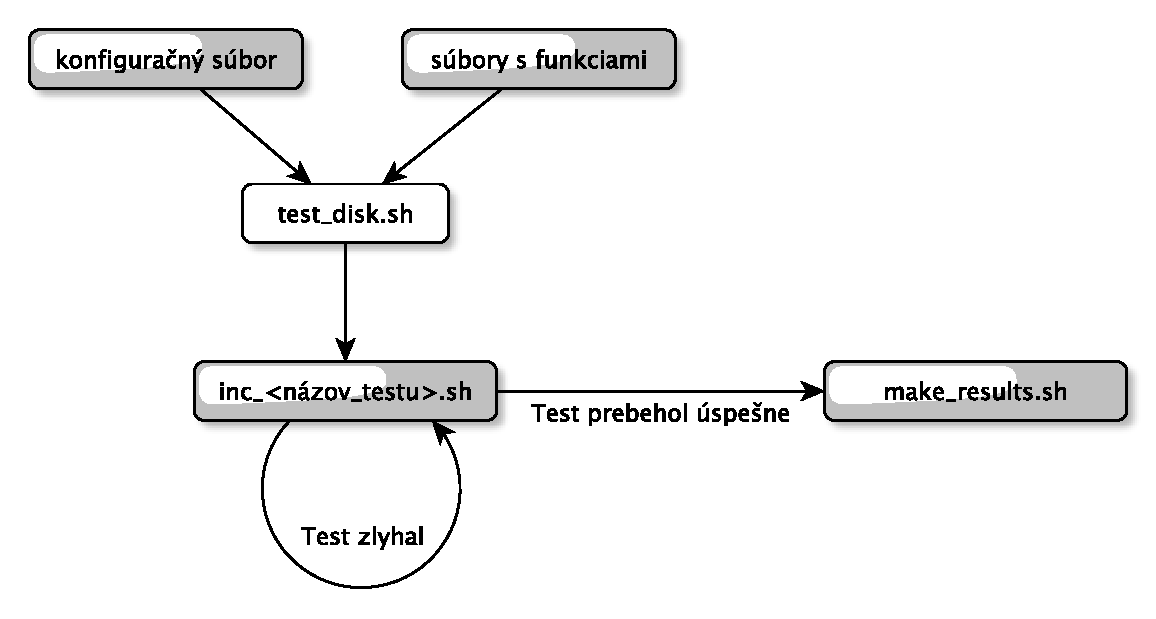
\includegraphics[width=\paperwidth-200pt]{data/testflow.pdf}}
  \caption{Priebeh testovania}
  \label{pic:testflow}
\end{center}
\end{figure}
%
% Test failing solving
%

\subsection{Riešenie problému so zlyhaním testu}
\label{sec:test-failure}

Test môže zlyhať z~nepredvídateľných príčin, ako je napríklad chyba
\emph{libvirt} popísaná v~kapitole \ref{sec:libvirt-problem}. Ak v~teste zlyhá
operácia, ktorá má vplyv na výsledky, zavolá sa funkcia \texttt{failedRunSave},
ktorá nastaví príznak chyby. Funkciou \texttt{failedRunCheck} vieme overiť
tento príznak. Ak napríklad nastala chyba pripájania diskov, test zápisu sa už
nespustí. Hlavný súbor \texttt{test\_disk.sh} taktiež využíva túto funkciu a
daný test opakovane spúšťa, ak je to potreba.

%
% Vysledky testovania
%

\chapter{Výsledky testovania}

\section{Automatizované spracovanie výsledkov}

Po skončení testov sa spúšťa skript \texttt{make\_results.sh}, ktorý
automatizovane spracováva výsledky testov a~generuje výstup vo formáte \LaTeX.
Výsledky sú v~tabuľkách a~rozdelené do sekcií. Ak chceme niektorú sekciu
dodatočne okomentovať, tento \LaTeX~kód očakáva dodatočné súbory s~menom
\texttt{obsah-test-<názov tuned profilu>.tex}. Ak tento súbor existuje, jeho
text sa vloží pre tabuľku s~výsledkami.


%
% Vyhodnotenie testov
%

\section{Vyhodnotenie testov}

% Nacitaj subory s vysledkami
\IfFileExists{test-results}{%
% START Automatic results
%
\subsection{Testovanie s profilom \emph{balanced}}
\IfFileExists{obsah-test-balanced}{Profil \emph{balanced} je prednastavený po spustení \emph{tuned}. Mal by
rovnomerne optimalizovať systém a je vhodným začiatkom pre bežnú prácu.

V základnom nastavení ale nerobí zásahy do diskov, ale iba \emph{CPU},
\emph{audio} a \emph{video}. Pre ladenie diskov by bolo potrebné ho upraviť,
ale toto testovanie sa zaoberá základnými profilmi.

Rozdiely v rýchlosti diskových operácií su preto minimálne a celkovo je rozdiel
iba v jednotkách percent.
}{}

\begin{table}[H]
\begin{center}
\begin{tabular}{|l|r r r r|}
    \hline
    \textbf{Test} & \textbf{bez tuned} & \textbf{s tuned} & \textbf{rozdiel} & \textbf{rozdiel [\%]} \\
    \hline & \\[-1em]\hline
    simple\_disk ext3 & 105\,s & 107\,s & -2\,s & -1.90\,\% \\
    raid0 ext3 & 117\,s & 117\,s & 0\,s & 0\,\% \\
    raid1 ext3 & 108\,s & 119\,s & -11\,s & -10.18\,\% \\
    \hline
    \textbf{Priemery} & \textbf{110.00 s}\,& \textbf{114.33\,s} & \textbf{-4.33\,s} & \textbf{-3.67\,\%} \\
    \hline & \\[-1em]\hline
    simple\_disk ext2 & 123\,s & 121\,s & 2\,s & 1.63\,\% \\
    raid0 ext2 & 116\,s & 120\,s & -4\,s & -3.44\,\% \\
    raid1 ext2 & 121\,s & 121\,s & 0\,s & 0\,\% \\
    \hline
    \textbf{Priemery} & \textbf{120.00 s}\,& \textbf{120.67\,s} & \textbf{-0.67\,s} & \textbf{-0.33\,\%} \\
    \hline & \\[-1em]\hline
    simple\_disk ext4 & 117\,s & 117\,s & 0\,s & 0\,\% \\
    raid0 ext4 & 114\,s & 116\,s & -2\,s & -1.75\,\% \\
    raid1 ext4 & 118\,s & 120\,s & -2\,s & -1.69\,\% \\
    \hline
    \textbf{Priemery} & \textbf{116.33 s}\,& \textbf{117.67\,s} & \textbf{-1.33\,s} & \textbf{-0.67\,\%} \\
    \hline & \\[-1em]\hline
    simple\_disk jfs & 123\,s & 122\,s & 1\,s & .82\,\% \\
    raid0 jfs & 123\,s & 118\,s & 5\,s & 4.07\,\% \\
    raid1 jfs & 129\,s & 131\,s & -2\,s & -1.55\,\% \\
    \hline
    \textbf{Priemery} & \textbf{125.00 s}\,& \textbf{123.67\,s} & \textbf{1.33\,s} & \textbf{1.67\,\%} \\
    \hline & \\[-1em]\hline
    simple\_disk reiserfs & 128\,s & 119\,s & 9\,s & 7.04\,\% \\
    raid0 reiserfs & 138\,s & 136\,s & 2\,s & 1.45\,\% \\
    raid1 reiserfs & 194\,s & 199\,s & -5\,s & -2.57\,\% \\
    \hline
    \textbf{Priemery} & \textbf{153.33 s}\,& \textbf{151.33\,s} & \textbf{2.00\,s} & \textbf{2.67\,\%} \\
    \hline & \\[-1em]\hline
    simple\_disk btrfs & 108\,s & 110\,s & -2\,s & -1.85\,\% \\
    raid0 btrfs & 123\,s & 116\,s & 7\,s & 5.70\,\% \\
    raid1 btrfs & 103\,s & 113\,s & -10\,s & -9.70\,\% \\
    \hline
    \textbf{Priemery} & \textbf{111.33 s}\,& \textbf{113.00\,s} & \textbf{-1.67\,s} & \textbf{-1.33\,\%} \\
    \hline & \\[-1em]\hline
    simple\_disk xfs & 105\,s & 108\,s & -3\,s & -2.85\,\% \\
    raid0 xfs & 113\,s & 111\,s & 2\,s & 1.77\,\% \\
    raid1 xfs & 116\,s & 116\,s & 0\,s & 0\,\% \\
    \hline
    \textbf{Priemery} & \textbf{111.33 s}\,& \textbf{111.67\,s} & \textbf{-0.33\,s} & \textbf{0.00\,\%} \\
    \hline & \\[-1em]\hline
    \textbf{Celkové priemery} & \textbf{121.76 s}\,& \textbf{121.76\,s} & \textbf{-0.71\,s} & \textbf{-0.24\,\%} \\
    \hline
\end{tabular}
\caption{Výsledky testov pre profil balanced}
\label{tab:results-xfs}
\end{center}
\end{table}

\subsection{Testovanie s profilom \emph{latency-performance}}
\IfFileExists{obsah-test-latency-performance}{Úlohou profilu \emph{latency-performance} je čo najviac znížiť latenciu
systému. Disky \texttt{sd*, cciss*, dm-*, vd*} sú ovplyvnené, ak je tento
profil aktívny. 

Rýchlosť diskových operácií sa zlepšila až o približne 8\,\%. Prekvapením je
experimentálny súborový systém \emph{btrfs}, ktorý pri použití s \emph{raid0}
zaznamenal zrýchlenie o viac ako 13\,\%.
}{}

\begin{table}[H]
\begin{center}
\begin{tabular}{|l|r r r r|}
    \hline
    \textbf{Test} & \textbf{bez tuned} & \textbf{s tuned} & \textbf{rozdiel} & \textbf{rozdiel [\%]} \\
    \hline & \\[-1em]\hline
    simple\_disk ext3 & 105\,s & 100\,s & 5\,s & 4.77\,\% \\
    raid0 ext3 & 117\,s & 107\,s & 10\,s & 8.55\,\% \\
    raid1 ext3 & 108\,s & 107\,s & 1\,s & .93\,\% \\
    \hline
    \textbf{Priemery} & \textbf{110.00 s}\,& \textbf{104.67\,s} & \textbf{5.33\,s} & \textbf{5.00\,\%} \\
    \hline & \\[-1em]\hline
    simple\_disk ext2 & 123\,s & 99\,s & 24\,s & 19.52\,\% \\
    raid0 ext2 & 116\,s & 111\,s & 5\,s & 4.32\,\% \\
    raid1 ext2 & 121\,s & 113\,s & 8\,s & 6.62\,\% \\
    \hline
    \textbf{Priemery} & \textbf{120.00 s}\,& \textbf{107.67\,s} & \textbf{12.33\,s} & \textbf{10.67\,\%} \\
    \hline & \\[-1em]\hline
    simple\_disk ext4 & 117\,s & 97\,s & 20\,s & 17.10\,\% \\
    raid0 ext4 & 114\,s & 104\,s & 10\,s & 8.78\,\% \\
    raid1 ext4 & 118\,s & 110\,s & 8\,s & 6.78\,\% \\
    \hline
    \textbf{Priemery} & \textbf{116.33 s}\,& \textbf{103.67\,s} & \textbf{12.67\,s} & \textbf{11.33\,\%} \\
    \hline & \\[-1em]\hline
    simple\_disk jfs & 123\,s & 110\,s & 13\,s & 10.57\,\% \\
    raid0 jfs & 123\,s & 118\,s & 5\,s & 4.07\,\% \\
    raid1 jfs & 129\,s & 111\,s & 18\,s & 13.96\,\% \\
    \hline
    \textbf{Priemery} & \textbf{125.00 s}\,& \textbf{113.00\,s} & \textbf{12.00\,s} & \textbf{10.00\,\%} \\
    \hline & \\[-1em]\hline
    simple\_disk reiserfs & 128\,s & 134\,s & -6\,s & -4.68\,\% \\
    raid0 reiserfs & 138\,s & 136\,s & 2\,s & 1.45\,\% \\
    raid1 reiserfs & 194\,s & 166\,s & 28\,s & 14.44\,\% \\
    \hline
    \textbf{Priemery} & \textbf{153.33 s}\,& \textbf{145.33\,s} & \textbf{8.00\,s} & \textbf{4.33\,\%} \\
    \hline & \\[-1em]\hline
    simple\_disk btrfs & 108\,s & 100\,s & 8\,s & 7.41\,\% \\
    raid0 btrfs & 123\,s & 106\,s & 17\,s & 13.83\,\% \\
    raid1 btrfs & 103\,s & 96\,s & 7\,s & 6.80\,\% \\
    \hline
    \textbf{Priemery} & \textbf{111.33 s}\,& \textbf{100.67\,s} & \textbf{10.67\,s} & \textbf{9.67\,\%} \\
    \hline & \\[-1em]\hline
    simple\_disk xfs & 105\,s & 94\,s & 11\,s & 10.48\,\% \\
    raid0 xfs & 113\,s & 110\,s & 3\,s & 2.66\,\% \\
    raid1 xfs & 116\,s & 109\,s & 7\,s & 6.04\,\% \\
    \hline
    \textbf{Priemery} & \textbf{111.33 s}\,& \textbf{104.33\,s} & \textbf{7.00\,s} & \textbf{7.00\,\%} \\
    \hline & \\[-1em]\hline
    \textbf{Celkové priemery} & \textbf{111.33 s}\,& \textbf{111.33\,s} & \textbf{9.71\,s} & \textbf{8.29\,\%} \\
    \hline
\end{tabular}
\caption{Výsledky testov pre profil latency-performance}
\label{tab:results-xfs}
\end{center}
\end{table}

\subsection{Testovanie s profilom \emph{powersave}}
\IfFileExists{obsah-test-powersave}{Ak potrebujeme ušetrit energiu, profil \emph{powersave} je na to najvhodnejší.
Na rýchlosť diskových operácií má ale negatívny efekt. Jeho aktivovaním sa
nastaví hodnota ALPM\footnote{Aggressive Link Power Management - technika,
ktorá pomáha šetriť energiu. Má tri stavy: min\_power, medium\_power a
max\_performance} na \texttt{min\_power}.

Výsledky sú približne totožné, ako s vypnutým \emph{tuned}. V niektorých
prípadoch sú dokonca horšie.
}{}

\begin{table}[H]
\begin{center}
\begin{tabular}{|l|r r r r|}
    \hline
    \textbf{Test} & \textbf{bez tuned} & \textbf{s tuned} & \textbf{rozdiel} & \textbf{rozdiel [\%]} \\
    \hline & \\[-1em]\hline
    simple\_disk ext3 & 105\,s & 108\,s & -3\,s & -2.85\,\% \\
    raid0 ext3 & 117\,s & 112\,s & 5\,s & 4.28\,\% \\
    raid1 ext3 & 108\,s & 126\,s & -18\,s & -16.66\,\% \\
    \hline
    \textbf{Priemery} & \textbf{110.00 s}\,& \textbf{115.33\,s} & \textbf{-5.33\,s} & \textbf{-4.33\,\%} \\
    \hline & \\[-1em]\hline
    simple\_disk ext2 & 123\,s & 118\,s & 5\,s & 4.07\,\% \\
    raid0 ext2 & 116\,s & 111\,s & 5\,s & 4.32\,\% \\
    raid1 ext2 & 121\,s & 125\,s & -4\,s & -3.30\,\% \\
    \hline
    \textbf{Priemery} & \textbf{120.00 s}\,& \textbf{118.00\,s} & \textbf{2.00\,s} & \textbf{2.33\,\%} \\
    \hline & \\[-1em]\hline
    simple\_disk ext4 & 117\,s & 113\,s & 4\,s & 3.42\,\% \\
    raid0 ext4 & 114\,s & 118\,s & -4\,s & -3.50\,\% \\
    raid1 ext4 & 118\,s & 127\,s & -9\,s & -7.62\,\% \\
    \hline
    \textbf{Priemery} & \textbf{116.33 s}\,& \textbf{119.33\,s} & \textbf{-3.00\,s} & \textbf{-2.00\,\%} \\
    \hline & \\[-1em]\hline
    simple\_disk jfs & 123\,s & 119\,s & 4\,s & 3.26\,\% \\
    raid0 jfs & 123\,s & 119\,s & 4\,s & 3.26\,\% \\
    raid1 jfs & 129\,s & 134\,s & -5\,s & -3.87\,\% \\
    \hline
    \textbf{Priemery} & \textbf{125.00 s}\,& \textbf{124.00\,s} & \textbf{1.00\,s} & \textbf{1.67\,\%} \\
    \hline & \\[-1em]\hline
    simple\_disk reiserfs & 128\,s & 166\,s & -38\,s & -29.68\,\% \\
    raid0 reiserfs & 138\,s & 142\,s & -4\,s & -2.89\,\% \\
    raid1 reiserfs & 194\,s & 151\,s & 43\,s & 22.17\,\% \\
    \hline
    \textbf{Priemery} & \textbf{153.33 s}\,& \textbf{153.00\,s} & \textbf{0.33\,s} & \textbf{-2.67\,\%} \\
    \hline & \\[-1em]\hline
    simple\_disk btrfs & 108\,s & 111\,s & -3\,s & -2.77\,\% \\
    raid0 btrfs & 123\,s & 118\,s & 5\,s & 4.07\,\% \\
    raid1 btrfs & 103\,s & 101\,s & 2\,s & 1.95\,\% \\
    \hline
    \textbf{Priemery} & \textbf{111.33 s}\,& \textbf{110.00\,s} & \textbf{1.33\,s} & \textbf{1.67\,\%} \\
    \hline & \\[-1em]\hline
    simple\_disk xfs & 105\,s & 107\,s & -2\,s & -1.90\,\% \\
    raid0 xfs & 113\,s & 124\,s & -11\,s & -9.73\,\% \\
    raid1 xfs & 116\,s & 115\,s & 1\,s & .87\,\% \\
    \hline
    \textbf{Priemery} & \textbf{111.33 s}\,& \textbf{115.33\,s} & \textbf{-4.00\,s} & \textbf{-3.00\,\%} \\
    \hline & \\[-1em]\hline
    \textbf{Celkové priemery} & \textbf{122.14 s}\,& \textbf{122.14\,s} & \textbf{-1.10\,s} & \textbf{-0.90\,\%} \\
    \hline
\end{tabular}
\caption{Výsledky testov pre profil powersave}
\label{tab:results-xfs}
\end{center}
\end{table}

\subsection{Testovanie s profilom \emph{throughput-performance}}
\IfFileExists{obsah-test-throughput-performance}{Tento profil ovplyvňuje disky podobne ako \emph{latency-performance}. Veľkým
rozdielom ale je v \emph{transparent huge pages}, ktoré
\emph{latency-performance} nastavuje na \texttt{never} a
\emph{throughput-performance} na \texttt{always}.

Zrýchlenie diskových operácií s týmto profilom dosajue hodnoty cez 10 \% a tým
sa stáva ideálnym profilom, ak chceme optimalizovať prácu s diskami.
}{}

\begin{table}[H]
\begin{center}
\begin{tabular}{|l|r r r r|}
    \hline
    \textbf{Test} & \textbf{bez tuned} & \textbf{s tuned} & \textbf{rozdiel} & \textbf{rozdiel [\%]} \\
    \hline & \\[-1em]\hline
    simple\_disk ext3 & 105\,s & 100\,s & 5\,s & 4.77\,\% \\
    raid0 ext3 & 117\,s & 107\,s & 10\,s & 8.55\,\% \\
    raid1 ext3 & 108\,s & 116\,s & -8\,s & -7.40\,\% \\
    \hline
    \textbf{Priemery} & \textbf{110.00 s}\,& \textbf{107.67\,s} & \textbf{2.33\,s} & \textbf{2.33\,\%} \\
    \hline & \\[-1em]\hline
    simple\_disk ext2 & 123\,s & 105\,s & 18\,s & 14.64\,\% \\
    raid0 ext2 & 116\,s & 110\,s & 6\,s & 5.18\,\% \\
    raid1 ext2 & 121\,s & 119\,s & 2\,s & 1.66\,\% \\
    \hline
    \textbf{Priemery} & \textbf{120.00 s}\,& \textbf{111.33\,s} & \textbf{8.67\,s} & \textbf{7.67\,\%} \\
    \hline & \\[-1em]\hline
    simple\_disk ext4 & 117\,s & 100\,s & 17\,s & 14.53\,\% \\
    raid0 ext4 & 114\,s & 108\,s & 6\,s & 5.27\,\% \\
    raid1 ext4 & 118\,s & 113\,s & 5\,s & 4.24\,\% \\
    \hline
    \textbf{Priemery} & \textbf{116.33 s}\,& \textbf{107.00\,s} & \textbf{9.33\,s} & \textbf{8.67\,\%} \\
    \hline & \\[-1em]\hline
    simple\_disk jfs & 123\,s & 106\,s & 17\,s & 13.83\,\% \\
    raid0 jfs & 123\,s & 104\,s & 19\,s & 15.45\,\% \\
    raid1 jfs & 129\,s & 108\,s & 21\,s & 16.28\,\% \\
    \hline
    \textbf{Priemery} & \textbf{125.00 s}\,& \textbf{106.00\,s} & \textbf{19.00\,s} & \textbf{15.67\,\%} \\
    \hline & \\[-1em]\hline
    simple\_disk reiserfs & 128\,s & 123\,s & 5\,s & 3.91\,\% \\
    raid0 reiserfs & 138\,s & 136\,s & 2\,s & 1.45\,\% \\
    raid1 reiserfs & 194\,s & 156\,s & 38\,s & 19.59\,\% \\
    \hline
    \textbf{Priemery} & \textbf{153.33 s}\,& \textbf{138.33\,s} & \textbf{15.00\,s} & \textbf{8.67\,\%} \\
    \hline & \\[-1em]\hline
    simple\_disk btrfs & 108\,s & 102\,s & 6\,s & 5.56\,\% \\
    raid0 btrfs & 123\,s & 107\,s & 16\,s & 13.01\,\% \\
    raid1 btrfs & 103\,s & 90\,s & 13\,s & 12.63\,\% \\
    \hline
    \textbf{Priemery} & \textbf{111.33 s}\,& \textbf{99.67\,s} & \textbf{11.67\,s} & \textbf{11.00\,\%} \\
    \hline & \\[-1em]\hline
    simple\_disk xfs & 105\,s & 97\,s & 8\,s & 7.62\,\% \\
    raid0 xfs & 113\,s & 102\,s & 11\,s & 9.74\,\% \\
    raid1 xfs & 116\,s & 107\,s & 9\,s & 7.76\,\% \\
    \hline
    \textbf{Priemery} & \textbf{111.33 s}\,& \textbf{102.00\,s} & \textbf{9.33\,s} & \textbf{8.67\,\%} \\
    \hline & \\[-1em]\hline
    \textbf{Celkové priemery} & \textbf{110.29 s}\,& \textbf{110.29\,s} & \textbf{10.76\,s} & \textbf{8.95\,\%} \\
    \hline
\end{tabular}
\caption{Výsledky testov pre profil throughput-performance}
\label{tab:results-xfs}
\end{center}
\end{table}

\subsection{Testovanie s profilom \emph{virtual-guest}}
\IfFileExists{obsah-test-virtual-guest}{\emph{Virtual-guest} by mal byť najvhodnejší profil pre virtuálny systém -- to
znamená, aj pre naše testovacie prostredie. Na diskoch upravuje
\emph{readahead} hodnotu a nastavuje ju na 4 krát väčšiu. Je ale dobré vedieť,
že taktiež zároveň načítava nastavenia z profilu \emph{throughput-performance}.

Práve pri tomto profile su najviac viditeľné rozdiely medzi súborovými
systémami. S použítím \emph{ext3} sme dosiahli zrýchlenie niečo cez 1\,\%, ale s
použitím \emph{ext2} je to až cez 10\,\%.

Toto nastavenie taktiež môžeme označiť za veľmi vhodné pre zrýchlenie diskových
operácií a znova je najväčšie zrýchlenie pri použití s \emph{JFS}, ale
najrýchlejší pri použítí kombinácie \emph{btrfs} a \emph{raid1} ako aj v
predchádzajúcom prípade. 
}{}

\begin{table}[H]
\begin{center}
\begin{tabular}{|l|r r r r|}
    \hline
    \textbf{Test} & \textbf{bez tuned} & \textbf{s tuned} & \textbf{rozdiel} & \textbf{rozdiel [\%]} \\
    \hline & \\[-1em]\hline
    simple\_disk ext3 & 105\,s & 101\,s & 4\,s & 3.81\,\% \\
    raid0 ext3 & 117\,s & 109\,s & 8\,s & 6.84\,\% \\
    raid1 ext3 & 108\,s & 116\,s & -8\,s & -7.40\,\% \\
    \hline
    \textbf{Priemery} & \textbf{110.00 s}\,& \textbf{108.67\,s} & \textbf{1.33\,s} & \textbf{1.33\,\%} \\
    \hline & \\[-1em]\hline
    simple\_disk ext2 & 123\,s & 100\,s & 23\,s & 18.70\,\% \\
    raid0 ext2 & 116\,s & 109\,s & 7\,s & 6.04\,\% \\
    raid1 ext2 & 121\,s & 115\,s & 6\,s & 4.96\,\% \\
    \hline
    \textbf{Priemery} & \textbf{120.00 s}\,& \textbf{108.00\,s} & \textbf{12.00\,s} & \textbf{10.33\,\%} \\
    \hline & \\[-1em]\hline
    simple\_disk ext4 & 117\,s & 105\,s & 12\,s & 10.26\,\% \\
    raid0 ext4 & 114\,s & 105\,s & 9\,s & 7.90\,\% \\
    raid1 ext4 & 118\,s & 111\,s & 7\,s & 5.94\,\% \\
    \hline
    \textbf{Priemery} & \textbf{116.33 s}\,& \textbf{107.00\,s} & \textbf{9.33\,s} & \textbf{8.33\,\%} \\
    \hline & \\[-1em]\hline
    simple\_disk jfs & 123\,s & 98\,s & 25\,s & 20.33\,\% \\
    raid0 jfs & 123\,s & 115\,s & 8\,s & 6.51\,\% \\
    raid1 jfs & 129\,s & 118\,s & 11\,s & 8.53\,\% \\
    \hline
    \textbf{Priemery} & \textbf{125.00 s}\,& \textbf{110.33\,s} & \textbf{14.67\,s} & \textbf{12.33\,\%} \\
    \hline & \\[-1em]\hline
    simple\_disk reiserfs & 128\,s & 118\,s & 10\,s & 7.82\,\% \\
    raid0 reiserfs & 138\,s & 125\,s & 13\,s & 9.43\,\% \\
    raid1 reiserfs & 194\,s & 169\,s & 25\,s & 12.89\,\% \\
    \hline
    \textbf{Priemery} & \textbf{153.33 s}\,& \textbf{137.33\,s} & \textbf{16.00\,s} & \textbf{10.33\,\%} \\
    \hline & \\[-1em]\hline
    simple\_disk btrfs & 108\,s & 108\,s & 0\,s & 0\,\% \\
    raid0 btrfs & 123\,s & 105\,s & 18\,s & 14.64\,\% \\
    raid1 btrfs & 103\,s & 89\,s & 14\,s & 13.60\,\% \\
    \hline
    \textbf{Priemery} & \textbf{111.33 s}\,& \textbf{100.67\,s} & \textbf{10.67\,s} & \textbf{9.67\,\%} \\
    \hline & \\[-1em]\hline
    simple\_disk xfs & 105\,s & 94\,s & 11\,s & 10.48\,\% \\
    raid0 xfs & 113\,s & 104\,s & 9\,s & 7.97\,\% \\
    raid1 xfs & 116\,s & 107\,s & 9\,s & 7.76\,\% \\
    \hline
    \textbf{Priemery} & \textbf{111.33 s}\,& \textbf{101.67\,s} & \textbf{9.67\,s} & \textbf{9.00\,\%} \\
    \hline & \\[-1em]\hline
    \textbf{Celkové priemery} & \textbf{110.52 s}\,& \textbf{110.52\,s} & \textbf{10.52\,s} & \textbf{8.76\,\%} \\
    \hline
\end{tabular}
\caption{Výsledky testov pre profil virtual-guest}
\label{tab:results-xfs}
\end{center}
\end{table}

%
% END Automatic results
%

}{}

%
% Bocné produkty
%

\chapter{Bočné produkty práce}

%
% Libvirt problemy
%

\section{Problém s~\emph{libvirtd}}
\label{sec:libvirt-problem}

Pri pripájaní diskov k~virtuálnemu systému za použitia príkazu \texttt{virsh
attach-device }, sa systém občas náhodne vypne. Nepodarilo sa mi spoľahlivo
zreprodukovať túto chybu do takého stavu, aby som ju mohol nahlásiť vývojárom,
pretože nastávala nepravidelne. 

O páde systému som nenašiel žiadnu zmienku v~logoch virtualizovaného ani
hostovacieho systému. 

Tento problém som riešil tým, že kontrolujem úspešnosť operácií a~test sa
automaticky opakuje, kým neskončí korektne. Táto problematika je presnejšie
popísaná v~kapitole \ref{sec:test-failure}.

%
% Power Management testday
%

\section{Power Management Test Day}

Dňa 17. apríla 2013 sa konal deň otvorených dverí Brnenskej pobočky firmy
\emph{Red Hat}. Súčasťou programu bol aj \emph{Power Management Test Day}
najnovšej verzie operačného systému \emph{Fedora 19}, ktorého som bol
spoluorganizátor. 

Mimo iné sa testovalo aj \emph{tuned} samotné. Najväčším prekvapením bolo
testovanie \emph{tuned} profilu \emph{powersave}, ktorý by mal znižovať
elektrický odber. Na testovanie prišlo množstvo ľudí s~rôznymi notebookmi.
Konkrétne výsledky sú uvedené v~tabuľke \ref{tab:testday-results}.

\begin{table}[H]
\begin{center}
\begin{tabular}{|l|r|r|r|}
    \hline
    \textbf{Typ notebooku} & \textbf{Odber bez tuned} & \textbf{Odber s~tuned} & \textbf{Zlepšenie} \\
    \hline
    Lenovo ThinkPad X230        & 4.540 Wh & 4.110 Wh & 9.47\% \\
    HP Elitebook 8540w          & 7.566 Wh & 7.493 Wh & 0.97\% \\
    Lenovo T60 laptop           & 4.720 Wh & 4.500 Wh & 4.66\% \\
    Dell Optiplex 990           & 8.500 Wh & 7.700 Wh & 9.41\% \\
    Lenovo ThinkPad T61         & 4.880 Wh & 4.340 Wh & 11.07\% \\
    Lenovo ThinkPad T520        & 5.387 Wh & 4.815 Wh & 10.62\% \\
    Lenovo T510                 & 3.310 Wh & 2.820 Wh & 14.80\% \\
    ThinkPad T430               & 5.690 Wh & 5.370 Wh & 5.62\% \\
    Samsung N210 (Intel Atom)   & 1.402 Wh & 1.394 Wh & 0.58\% \\
    \hline
    \textbf{Priemerné zlepšenie} & \multicolumn{3}{|r|}{7.47\%} \\
    \hline
\end{tabular}
\caption{Odber rôznych notebookov s~vypnutým a~zapnutým tuned.}
\label{tab:testday-results}
\end{center}
\end{table}

Už na prvý pohľad je viditeľné, že tento \emph{tuned} profil si robí svoju
prácu. V~priemere sa odber znížil o 7.47 \%. 

%
% Najdene chyby
%

\section{Nájdené chyby}

Počas písania tejto bakalárskej práce, narábanie s~\emph{tuned} a~testovaní som
narazil na niekoľko chýb, ktoré som nahlasoval do oficiálnej \emph{Red Hat} a
\emph{Fedora} bugzilly~\cite{rhBugzilla}. Chyby sa nachádzali väčšinou priamo v
balíku \emph{tuned}, ale taktiež v~balíku \emph{selinux-policy}.

Tieto chyby boli väčśinou opravené do pár dní. Ich prehľad je v~tabuľke \ref{tab:bugs}.

\begin{table}[H]
\begin{center}
\begin{tabular}{|l|l|l|}
    \hline
    \textbf{Číslo chyby} & \textbf{Názov} & \textbf{Status} \\
    \hline
    BZ\#907065 & tuned-adm can crash because of unknown variable log & opravené \\
    BZ\#953128 & tuned does not start if active profile is missing & opravené \\
    BZ\#953132 & AVCs after starting tuned daemon & opravené \\
    BZ\#901689 & Typo in tuned-adm.py & opravené \\
    BZ\#911138 & tuned-adm profile virtual-guest/host AVC denied & zatiaľ neopravené \\
    BZ\#958575 & mkfs.btrfs segfaults & opravené \\
    \hline
\end{tabular}
\caption{Zoznam nájdených chýb}
\label{tab:bugs}
\end{center}
\end{table}

Tieto chyby neovplyvnili testovanie, pretože neboli až tak závažné alebo ich
vývojár rýchlo opravil. Jedine chyba v~\texttt{mkfs.btrfs} znemožnila
testovanie na súborovom systéme \emph{btrfs}.


%
% Zaver 
%

\chapter{Záver}

Z výsledkov je jasné, že \emph{tuned} naozaj optimalizuje I/O operácie na
diskových poliach. 

%
% Prilohy
%

\setcounter{chapter}{0}
\renewcommand{\thechapter}{\Alph{chapter}}
\chapter{Príloha CD}

